\chapter{Sprint 1 – Authentication and Role Management}

\section{Introduction}

The first sprint focused on implementing secure user authentication and redirecting users to the appropriate interface based on their role. This sprint was essential for laying the groundwork of access control and system segmentation between cashiers and administrators.

The goal was to allow users to log in through a trusted identity provider (Auth0), verify their role securely, and then route them to the corresponding interface without exposing protected content to unauthorized users.

\section{Sprint 1 Backlog}

\begin{table}[H]
\centering
\begin{tabular}{|c|p{10cm}|c|}
\hline
\textbf{Task ID} & \textbf{Task Description} & \textbf{Status} \\
\hline
S1-T1 & Set up Auth0 authentication & Completed \\
S1-T2 & Create user roles system & Completed \\
S1-T3 & Build login redirection & Completed \\
S1-T4 & Protect routes by role & Completed \\
\hline
\end{tabular}
\caption{Sprint 1 – Backlog}
\label{tab:sprint1-backlog}
\end{table}

\section{Functional Specification}

The system implements a dual authentication approach to accommodate different user types and security requirements:

\begin{itemize}
  \item \textbf{Admin users:} Secure authentication via Auth0 OAuth provider with enhanced security features
  \item \textbf{Cashier users:} Local authentication system for faster access and simplified login process
\end{itemize}

Once authenticated, the application retrieves the user's role and conditionally renders either:

\begin{itemize}
  \item The cashier dashboard: a simple POS interface focused on transactions (local auth)
  \item The admin dashboard: an interface with access to management and analytics (Auth0)
\end{itemize}

Admin roles are determined using email-based matching or predefined metadata in Auth0, while cashier roles are managed through the local user database.

\section{Use Case Diagram}

\begin{figure}[H]
  \centering
  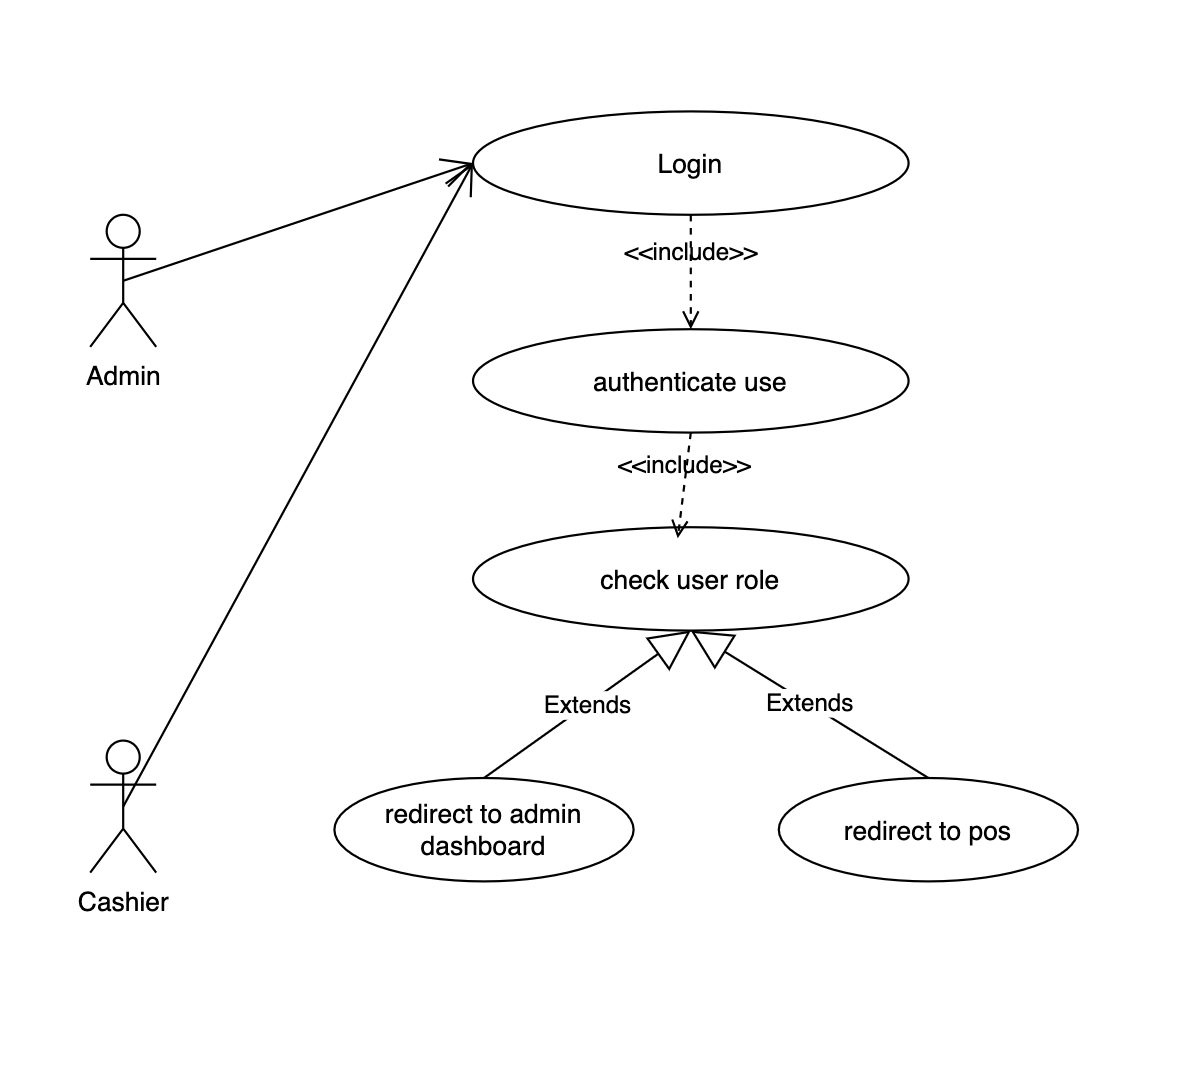
\includegraphics[width=0.9\textwidth]{figures/images/sprint1usecase.png}
  \caption{Sprint 1 – Authentication Use Case Diagram}
  \label{fig:sprint1-usecase}
\end{figure}

The authentication use case diagram identifies the interactions between users and the authentication system. Key use cases include:

\begin{itemize}
  \item User login with email and password
  \item Role-based redirection (Admin vs Cashier)
  \item Session management and logout
  \item Token validation and refresh
\end{itemize}

\section{Sequence Diagram}

\begin{figure}[H]
  \centering
  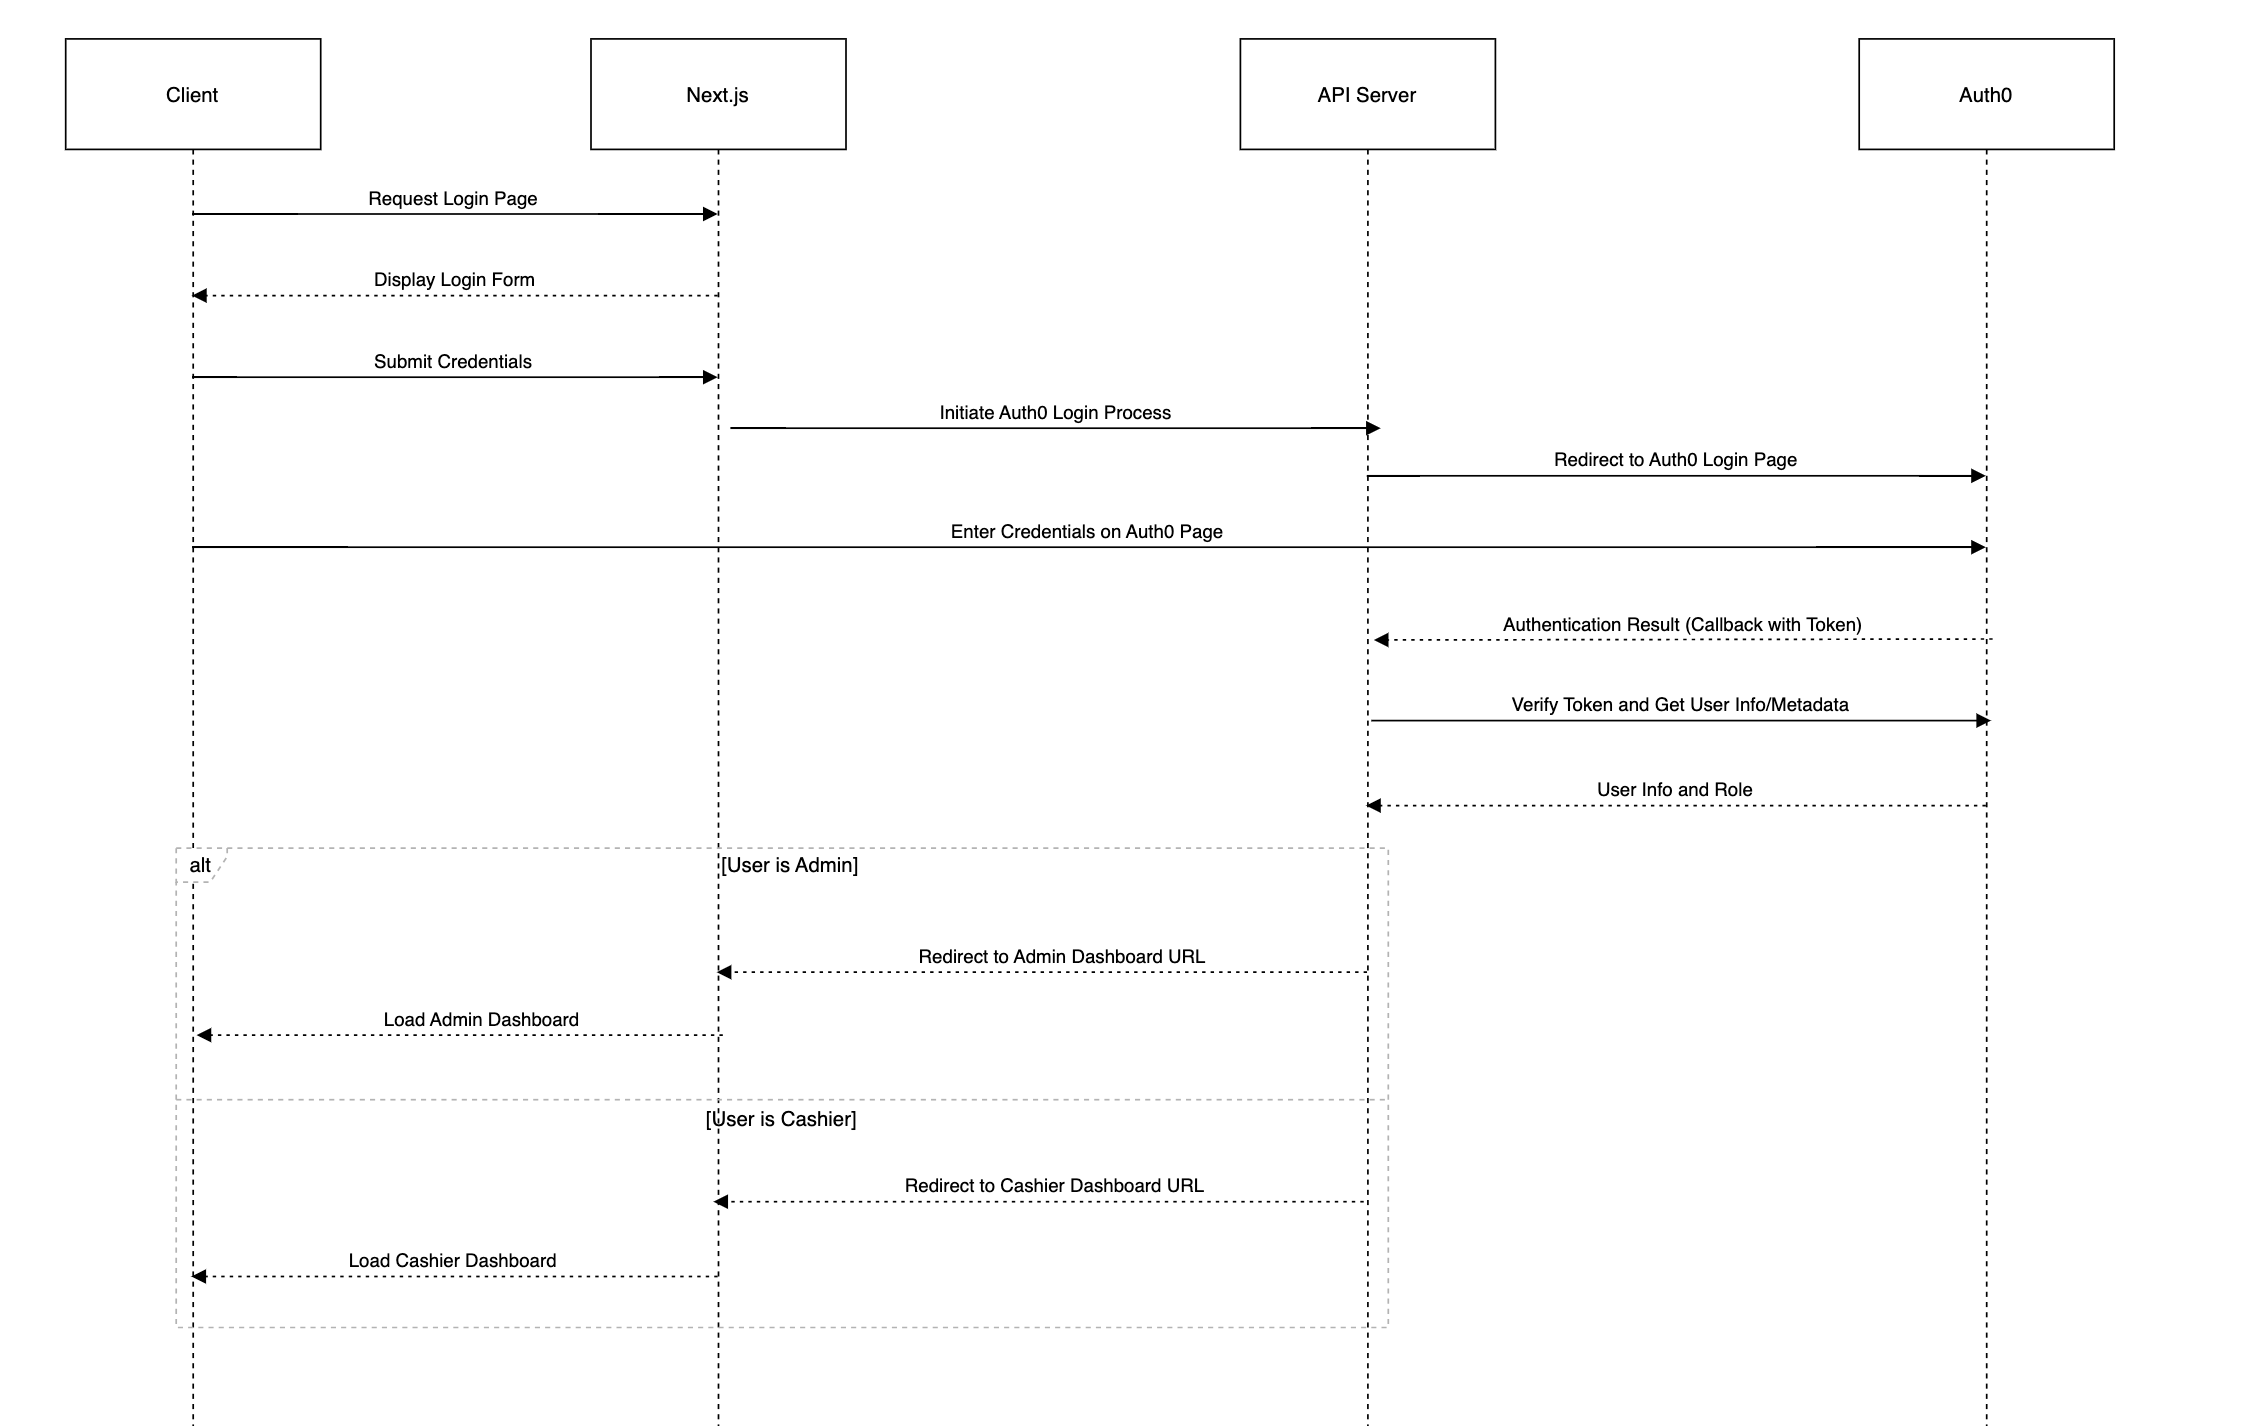
\includegraphics[width=0.9\textwidth]{figures/images/sprint1sequence.png}
  \caption{Sprint 1 – Authentication Sequence Diagram}
  \label{fig:sprint1-sequence}
\end{figure}

The login sequence follows these steps:
\begin{enumerate}
  \item User submits credentials to the login form
  \item \textbf{For Admin users:} Next.js API validates credentials with Auth0 OAuth provider
  \item \textbf{For Cashier users:} Next.js API validates credentials against local database
  \item Authentication provider returns token and user profile
  \item System determines user role and redirects accordingly
  \item User session is established and maintained
\end{enumerate}

\section{Implementation Highlights}

The integration process required implementing two distinct authentication flows to accommodate different user types and security requirements:

\subsection*{Dual Authentication System}

\textbf{Auth0 Integration for Admin Users:}
The Auth0 React SDK was used to enable secure OAuth login for administrators. After successful login, a JSON Web Token (JWT) is generated and used to verify the admin's identity across protected routes.

\textbf{Local Authentication for Cashiers:}
A custom local authentication system was implemented for cashier users, providing faster login access and simplified credential management suitable for point-of-sale operations.

\subsection*{Role Definition and Routing}

Each authenticated user is assigned a role based on their authentication method:
\begin{itemize}
  \item Admin users authenticated via Auth0 access management dashboards and analytics
  \item Cashier users authenticated locally access the POS interface
\end{itemize}

\subsection*{Protected Routes}

Using Next.js middleware and client-side checks, unauthorized access is prevented for both authentication types. The system validates tokens appropriately based on the authentication method used.

\subsection*{UI Feedback and Session Handling}

Sessions persist during browser refresh for both authentication types, and the logout process fully clears the user token. The interface adapts based on the authentication method and user role.

\section{Class Diagram}

\begin{figure}[H]
  \centering
  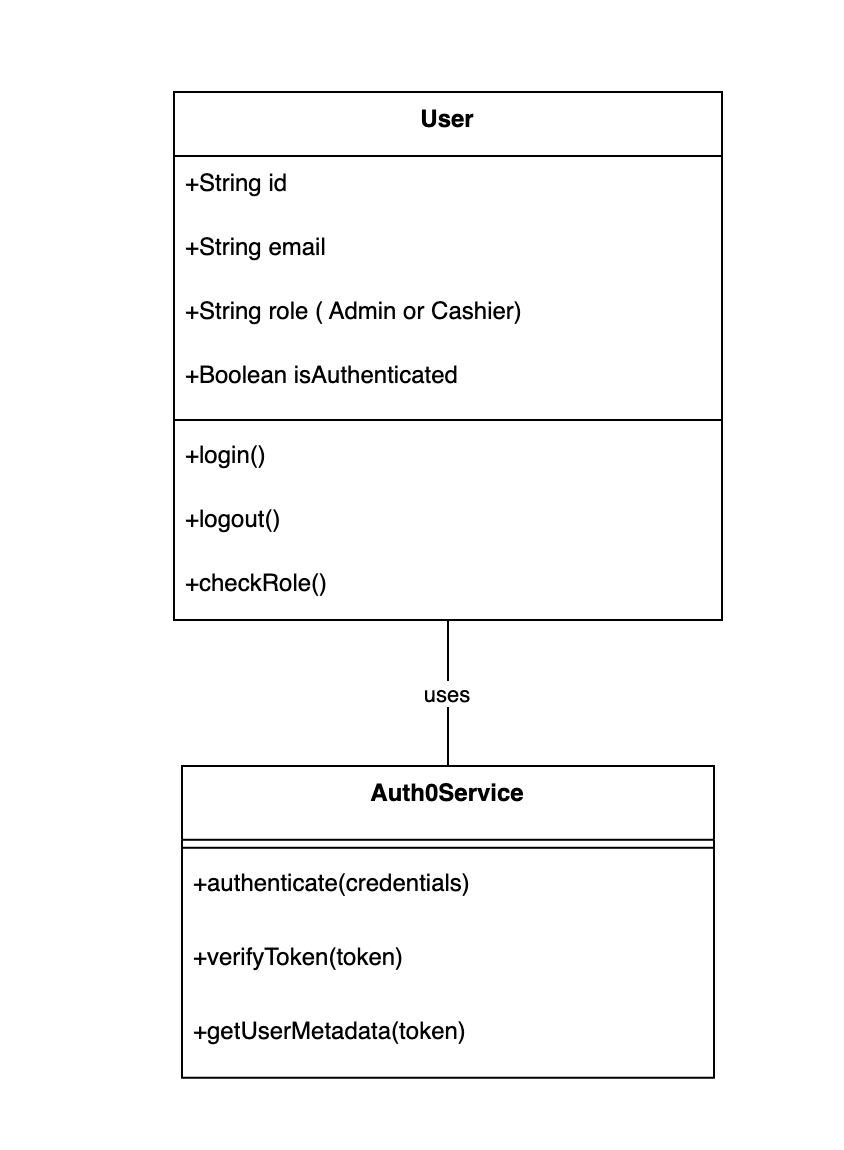
\includegraphics[width=0.9\textwidth]{figures/images/sprint1class.png}
  \caption{Sprint 1 – Authentication Class Diagram}
  \label{fig:sprint1-class}
\end{figure}

\section{Implementation Results}

% Login screen screenshot removed - to be replaced with new screenshot

The authentication system was successfully implemented with the following features:

\begin{itemize}
  \item Clean, responsive login interface supporting both authentication methods
  \item Secure credential validation through Auth0 for admin users
  \item Local authentication system for cashier users with optimized performance
  \item Automatic role-based redirection based on authentication type
  \item Session persistence across browser sessions for both user types
  \item Error handling for invalid credentials in both systems
  \item Loading states and user feedback adapted to authentication method
\end{itemize}

The dual authentication approach provides appropriate security levels for different user roles while maintaining optimal user experience for each user type.

\section{Testing and Results}

Manual testing was conducted on local builds to simulate both authentication methods and user roles. The following scenarios were verified:

\begin{itemize}
  \item Login as a cashier (local auth) → redirected to POS dashboard
  \item Login as an admin (Auth0) → redirected to admin dashboard
  \item Cross-authentication method validation and security
  \item Unauthorized access to /admin or /pos routes → blocked or redirected
  \item Logout from both authentication systems → session cleared and returned to login screen
\end{itemize}

\begin{figure}[H]
  \centering
  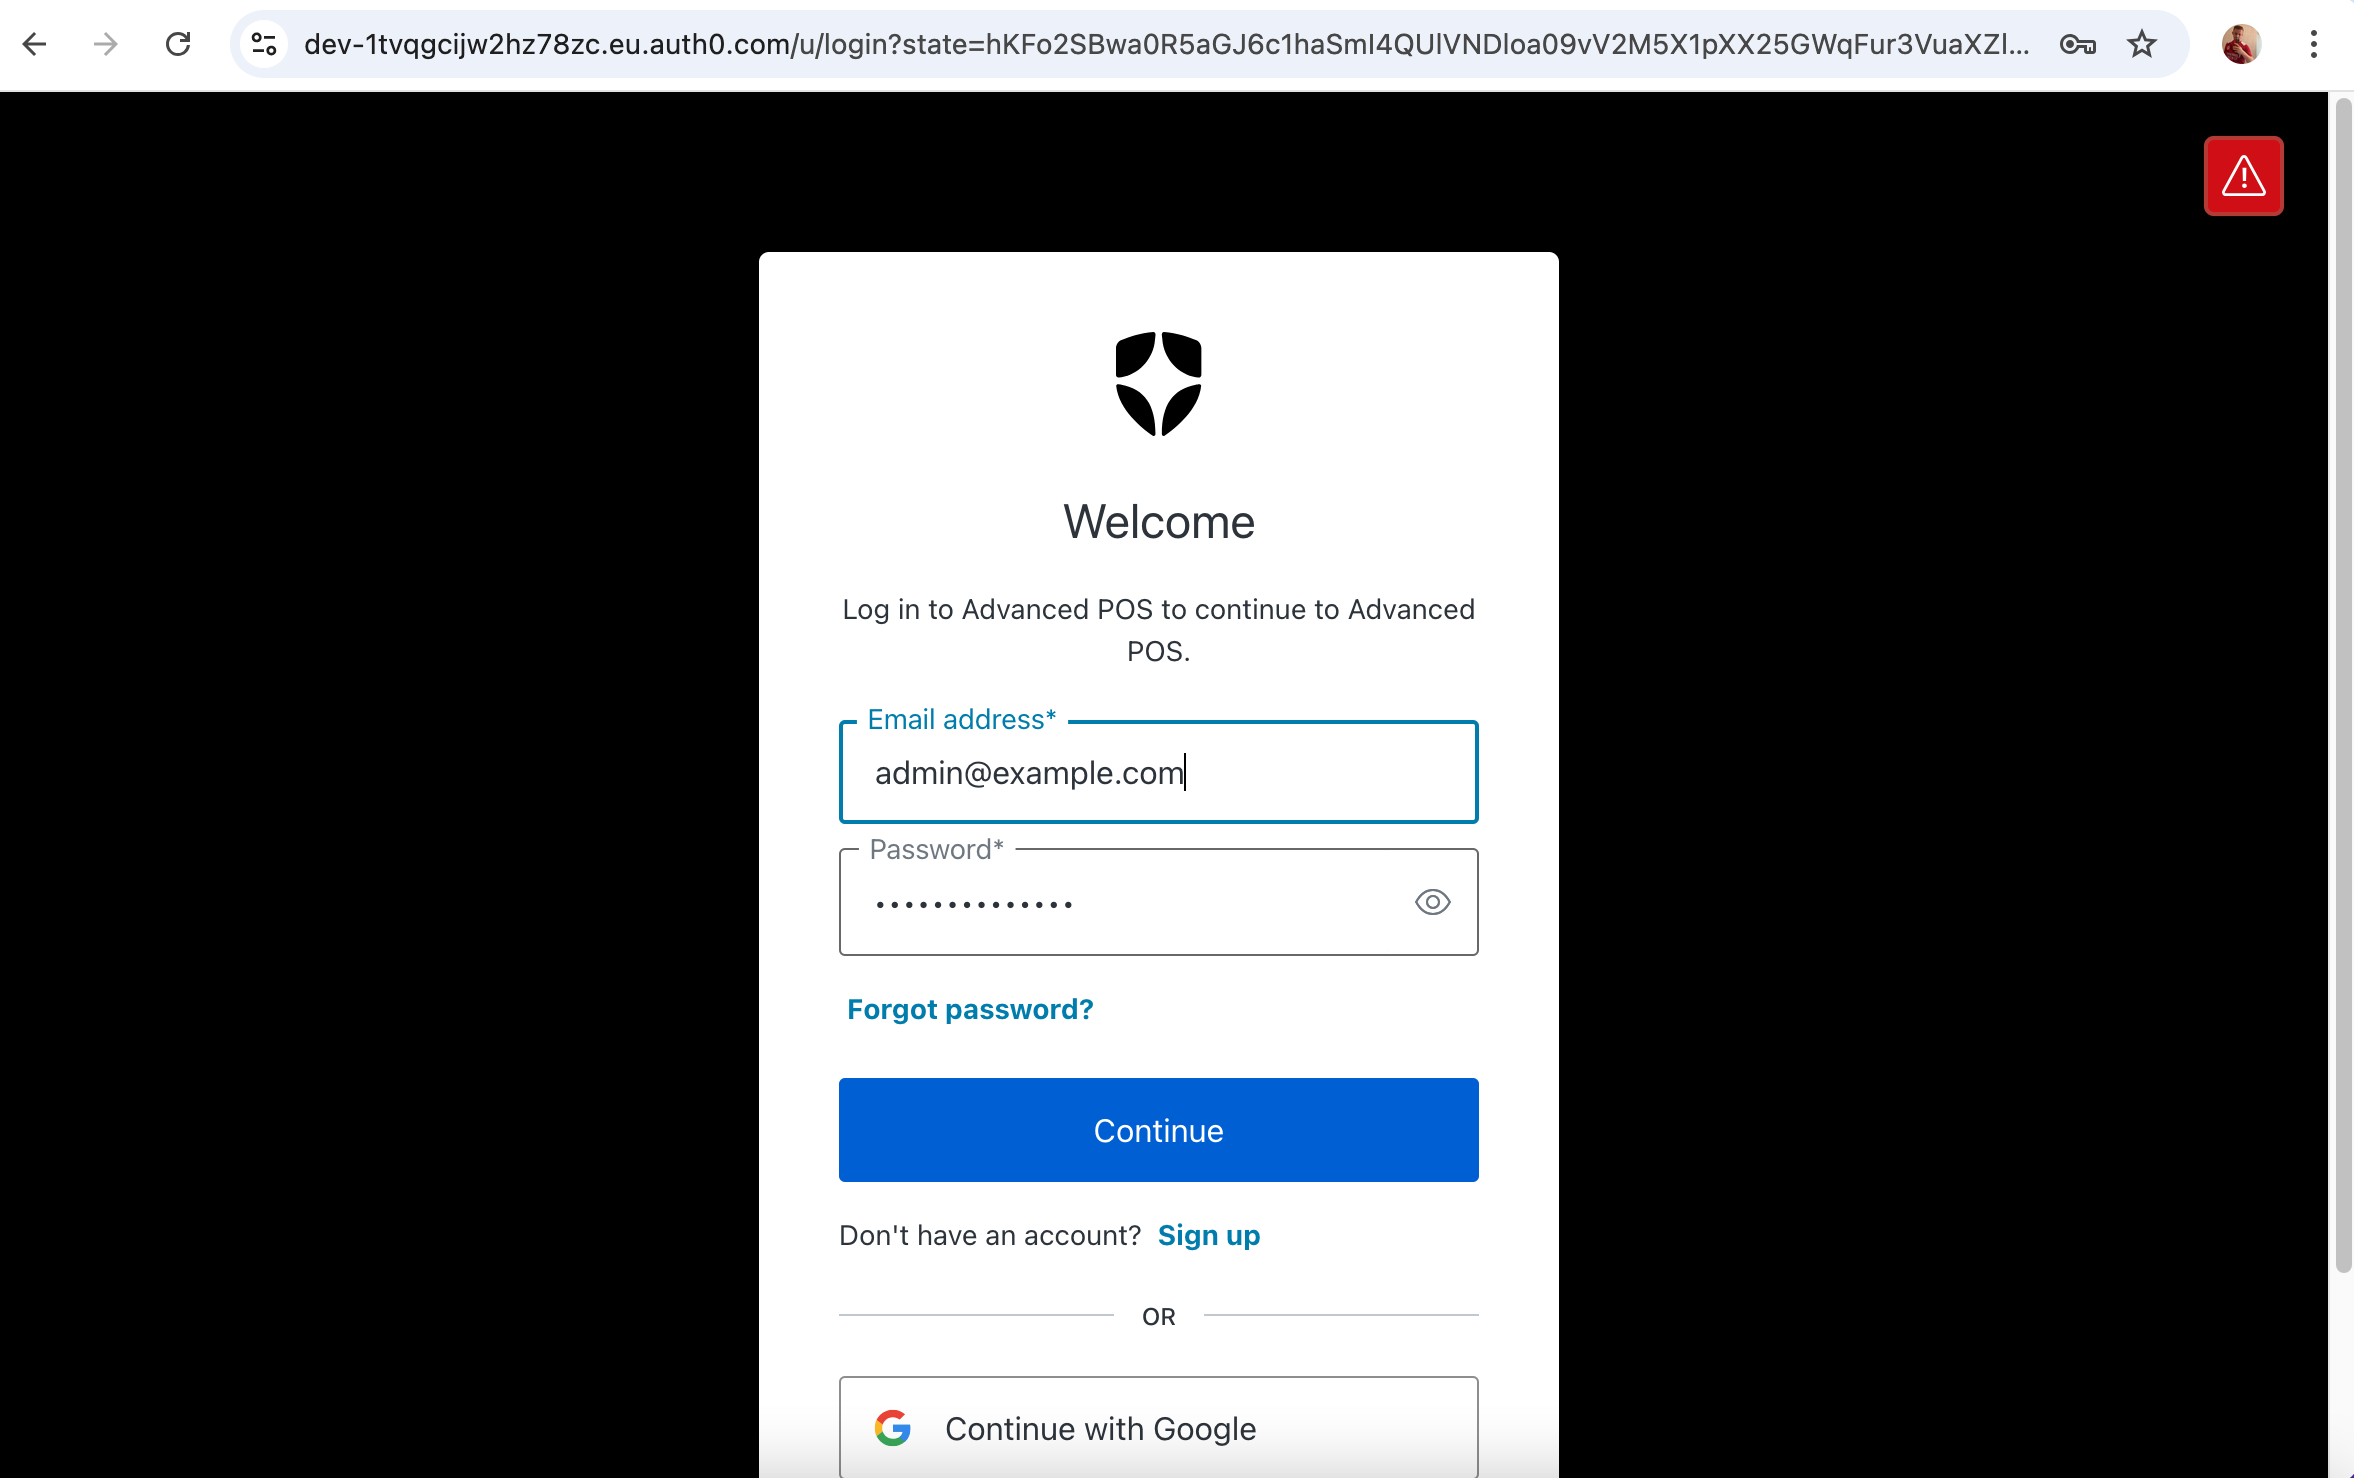
\includegraphics[width=0.9\textwidth]{working app screenshots/loginauth0.png}
  \caption{Login Interface – Auth0 Integration Test}
  \label{fig:sprint1-login}
\end{figure}

The authentication and routing system worked reliably throughout this sprint. No major issues were encountered once session persistence and route guards were in place.

\section{Conclusion}

Sprint 1 successfully delivered the core authentication layer and dynamic role-based routing logic. This functionality not only enhances security but also defines the foundation for all user interactions in later sprints. With user access in place, the next sprint will focus on building the main cashier interface and enabling product selection and transaction logic.
